\documentclass{../common/SCNU_Experimental_Report}

% 填写报告头信息
\studentname{汤承洲}
\studentid{20233902058}
\major{电子信息工程}
\class{23级2班}
\coursename{控制工程}
\projectname{综合练习}
\verify
\experimentdate{2026年6月16日}
\teacher{熊爱民}

\graphicspath{{./figures/}}

\begin{document}
\maketitle

\section{实验目的}
\begin{enumerate}
    \item 掌握部分分式展开方法，能使用MATLAB的\texttt{residue()}函数对有理传递函数进行展开，并能推导有源运算放大器网络的传递函数。
    \item 掌握控制系统时间域分析方法，能计算系统的单位脉冲响应和单位阶跃响应指标（上升时间、峰值时间、最大超调量、调节时间），并分析增益$K$对系统动态性能的影响。
    \item 掌握频域分析方法，能使用MATLAB绘制Bode图和Nyquist图，并读取稳定裕度。
    \item 掌握稳定裕度的概念和计算方法，能利用Bode图和Nyquist图判断系统的稳定性。
    \item 掌握PID控制器的设计方法，能通过相位裕度分析和极点配置法设计校正环节，改善系统性能。
    \item 掌握根轨迹分析方法，能绘制常规根轨迹和参量根轨迹，分析增益和反馈参数对系统闭环极点位置及动态性能的影响。
\end{enumerate}

\section{实验原理}
\subsection{部分分式展开与传递函数}
部分分式展开是将复杂有理传递函数分解为若干个简单分式之和的方法。MATLAB的\texttt{residue()}函数可计算有理分式的留数、极点和直项：
\[
\frac{N(s)}{D(s)} = \sum_{i=1}^{n} \frac{r_i}{s - p_i} + k(s)
\]
其中$r_i$为留数，$p_i$为极点，$k(s)$为直项（当分子阶次不低于分母阶次时存在）。

运算放大器电路利用"虚短"和"虚断"特性，通过阻抗网络实现各种传递函数。对于反相放大器结构，有$G(s) = -Z_f(s)/Z_i(s)$，其中$Z_f$为反馈阻抗，$Z_i$为输入阻抗。

\subsection{时间响应分析}
二阶系统的标准传递函数为：
\[
G(s) = \frac{\omega_n^2}{s^2 + 2\zeta\omega_n s + \omega_n^2}
\]
其中$\omega_n$为自然频率，$\zeta$为阻尼比。典型阶跃响应指标包括：
\begin{itemize}
    \item 上升时间$t_r$：响应从终值的10\%上升到90\%所需时间
    \item 峰值时间$t_p$：响应达到第一个峰值所需时间
    \item 最大超调量$M_p$：峰值超出终值的百分比
    \item 调节时间$t_s$：响应进入并保持在终值的$\pm$2\%（或$\pm$5\%）范围内所需时间
\end{itemize}

增益$K$影响闭环系统的阻尼比：$K$增大使阻尼比减小，响应加快但超调增大；$K$减小使阻尼比增大，响应变慢但更平稳。

\subsection{Bode图与Nyquist图}
Bode图由对数幅频特性曲线和相频特性曲线组成，横轴为角频率的对数刻度，纵轴分别为幅值（dB）和相位（度）。Nyquist图是在极坐标中绘制频率特性$G(j\omega)$随$\omega$从$0\to\infty$变化的轨迹，曲线的形状和与临界点$(-1, j0)$的关系可反映系统稳定性。

\subsection{稳定裕度}
稳定裕度衡量系统的相对稳定性，包括：
\begin{itemize}
    \item 幅值裕量$G_m$：系统在相位穿越频率$\omega_{cg}$处（相角为$-\pi$），幅值$|G(j\omega)|$的倒数，以dB表示时$G_m(\text{dB}) = -20\lg|G(j\omega_{cg})|$
    \item 相角裕量$P_m$：系统在幅值穿越频率$\omega_{cp}$处（幅值为1），相角与$-\pi$的差值
\end{itemize}
稳定系统要求$G_m > 1$（$G_m(\text{dB}) > 0$）且$P_m > 0^\circ$。

Nyquist稳定判据：若开环传递函数$G(s)$在右半$s$平面的极点数$P=0$，则闭环系统稳定的充要条件是Nyquist曲线不包围$(-1, j0)$点。

\subsection{PID控制器设计}
PID控制器的传递函数为：
\[
G_c(s) = K_p + \frac{K_i}{s} + K_d s
\]
其中$K_p$为比例系数，$K_i$为积分系数，$K_d$为微分系数。

极点配置法通过选择PID参数，使闭环系统的极点位于期望位置，从而获得预期的动态性能。对于三阶系统设计三个极点，通过特征多项式系数匹配求解PID参数。

\subsection{根轨迹分析}
根轨迹是当系统某一参数（通常为开环增益$K$）从$0$变化到$\infty$时，闭环特征方程的根在$s$平面上的轨迹。绘制依据是幅值条件和相角条件：
\[
|G(s)H(s)| = 1, \quad \angle G(s)H(s) = \pm 180^\circ(2k+1)
\]

参量根轨迹用于分析非增益参数（如反馈系数$K_h$）变化时系统极点轨迹，需将特征方程重写为等效开环传递函数形式。

\section{实验内容}
\subsection{Task 01：部分分式展开与传递函数（第2章）}

\subsubsection{例题2-27：部分分式展开}
对传递函数
\[
G(s) = \frac{s^4 + 11s^3 + 39s^2 + 52s + 26}{s^4 + 10s^3 + 35s^2 + 50s + 24}
\]
进行部分分式展开。使用\texttt{residue()}函数求得留数$r = [1, 2.5, -3, 0.5]$，极点$p = [-4, -3, -2, -1]$，直项$k = 1$。展开结果为：
\[
G(s) = 1 + \frac{1}{s+4} + \frac{2.5}{s+3} - \frac{3}{s+2} + \frac{0.5}{s+1}
\]

\subsubsection{习题2-11：有源电路网络传递函数}
推导四个运算放大器电路的传递函数，分别为：
\begin{itemize}
    \item 电路(a)：反相放大器，$R_2\|C$反馈，$G_a(s) = -\dfrac{R_2}{R_1(CR_2s+1)}$，为一阶惯性环节
    \item 电路(b)：反相放大器，$(R_2+C)\|R_4$反馈，$G_b(s) = -\dfrac{R_4(CR_2s+1)}{R_1(CR_2s+CR_4s+1)}$，含一阶超前因子
    \item 电路(c)：T型网络反馈，$G_c(s) = -\dfrac{R_2+R_4+CR_2R_4s}{R_1}$，为一阶比例-微分形式
    \item 电路(d)：复杂反馈网络（两个电容），$G_d(s)$为二阶有理分式，分子含$s$和$s^2$项
\end{itemize}

\subsection{Task 02：脉冲响应与阶跃响应分析（第3章）}

\subsubsection{例题3-5：单位脉冲响应}
系统传递函数为$G(s) = 50/(25s^2+2s+1)$。计算得自然频率$\omega_n = 0.2000$ rad/s，阻尼比$\zeta = 0.2000$。单位脉冲响应曲线如图\ref{fig:ex7_task02_01}所示，最大幅值为7.5604，出现在$t=6.9078$ s处。

\begin{figure}[H]
    \centering
    
\includegraphics[width=0.72\textwidth]{./figures/Task02_Figure_01.png}
    \caption{单位脉冲响应曲线（例题3-5）}
    \label{fig:ex7_task02_01}
\end{figure}

\subsubsection{习题3-7：阶跃响应指标与增益影响}
单位反馈系统开环传递函数$G(s) = 1/(s(s+1))$，闭环传递函数$T(s) = 1/(s^2+s+1)$。阶跃响应曲线如图\ref{fig:ex7_task02_02}所示，计算得各项指标：
\begin{itemize}
    \item 上升时间$t_r = 1.6390$ s
    \item 峰值时间$t_p = 3.5920$ s
    \item 最大超调量$M_p = 16.29$\%
    \item 调节时间$t_s = 8.0759$ s
\end{itemize}

\begin{figure}[H]
    \centering
    
\includegraphics[width=0.72\textwidth]{./figures/Task02_Figure_02.png}
    \caption{阶跃响应曲线（习题3-7，$K=1$）}
    \label{fig:ex7_task02_02}
\end{figure}

分析不同增益$K$对系统动态性能的影响，$K$分别取0.5、1、2、5、10，阶跃响应对比曲线如图\ref{fig:ex7_task02_03}所示，各项指标汇总于表\ref{tab:task02_k}。

\begin{figure}[H]
    \centering
    
\includegraphics[width=0.72\textwidth]{./figures/Task02_Figure_03.png}
    \caption{不同$K$值下的阶跃响应对比}
    \label{fig:ex7_task02_03}
\end{figure}

\begin{table}[H]
    \centering
    \caption{不同增益$K$的阶跃响应指标}
    \label{tab:task02_k}
    \small
    \begin{tabular}{ccccc}
        \toprule
        $K$ & 上升时间$t_r$ (s) & 峰值时间$t_p$ (s) & 超调量$M_p$ (\%) & 调节时间$t_s$ (s) \\
        \midrule
        0.5 & 3.0390 & 6.2630 & 4.32  & 8.4326 \\
        1.0 & 1.6390 & 3.5920 & 16.29 & 8.0759 \\
        2.0 & 0.9887 & 2.3947 & 30.49 & 7.7420 \\
        5.0 & 0.5533 & 1.4737 & 48.52 & 7.5607 \\
        10.0 & 0.3738 & 1.0131 & 60.45 & 7.3148 \\
        \bottomrule
    \end{tabular}
\end{table}

分析表明：随着$K$增大，系统响应加快（上升时间从3.0390s降至0.3738s），但超调量急剧增大（从4.32\%升至60.45\%），系统由过阻尼（$K=0.5$）经临界阻尼（$K=1$）过渡到欠阻尼状态（$K>1$），振荡加剧。

\subsection{Task 03：Bode图与Nyquist图（第4章）}

\subsubsection{例题4-8：Bode图}
系统$G(s) = 50/(25s^2+2s+1)$的Bode图如图\ref{fig:ex7_task03_01}所示。计算得幅值裕量$G_m = \infty$（无穷大），相角裕量$P_m = 3.2725^\circ$，增益穿越频率$\omega_{cp} = 1.4272$ rad/s。由于系统为二阶，相位永远不会到达$-\pi$，故幅值裕量为无穷大。

\begin{figure}[H]
    \centering
    
\includegraphics[width=0.72\textwidth]{./figures/Task03_Figure_01.png}
    \caption{Bode图（例题4-8）}
    \label{fig:ex7_task03_01}
\end{figure}

\subsubsection{例题4-10：Nyquist图}
系统的Nyquist图如图\ref{fig:ex7_task03_02}所示，局部放大图如图\ref{fig:ex7_task03_03}所示。Nyquist曲线不包围临界点$(-1, j0)$，系统稳定。

\begin{figure}[H]
    \centering
    
\includegraphics[width=0.72\textwidth]{./figures/Task03_Figure_02.png}
    \caption{Nyquist图（例题4-10）}
    \label{fig:ex7_task03_02}
\end{figure}

\begin{figure}[H]
    \centering
    
\includegraphics[width=0.72\textwidth]{./figures/Task03_Figure_03.png}
    \caption{Nyquist图局部放大}
    \label{fig:ex7_task03_03}
\end{figure}

\subsubsection{习题4-15：Nyquist图对比}
系统(1) $G(s) = 1/[(s+1)(2s+1)]$（图\ref{fig:ex7_task03_04}）和系统(2) $G(s) = 1/[s^2(s+1)(2s+1)]$（图\ref{fig:ex7_task03_05}）的Nyquist图对比如图\ref{fig:ex7_task03_06}所示。系统(1)为0型系统，Nyquist曲线起始于正实轴；系统(2)含两个积分环节（II型系统），曲线起始于负实轴无穷远处，在低频段有独特的相位特性。

\begin{figure}[H]
    \centering
    
\includegraphics[width=0.48\textwidth]{./figures/Task03_Figure_04.png}
    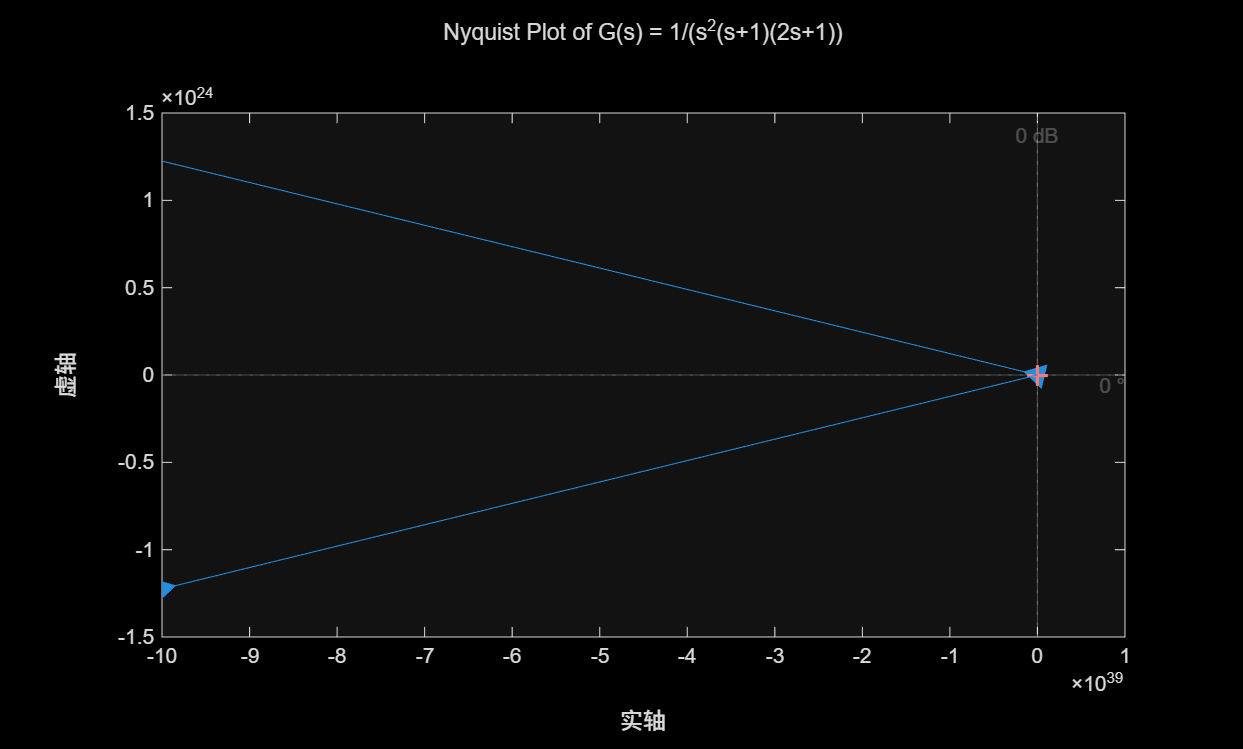
\includegraphics[width=0.48\textwidth]{./figures/Task03_Figure_05.png}
    \caption{(左) 系统(1) Nyquist图；(右) 系统(2) Nyquist图}
    \label{fig:ex7_task03_04_05}
\end{figure}

\begin{figure}[H]
    \centering
    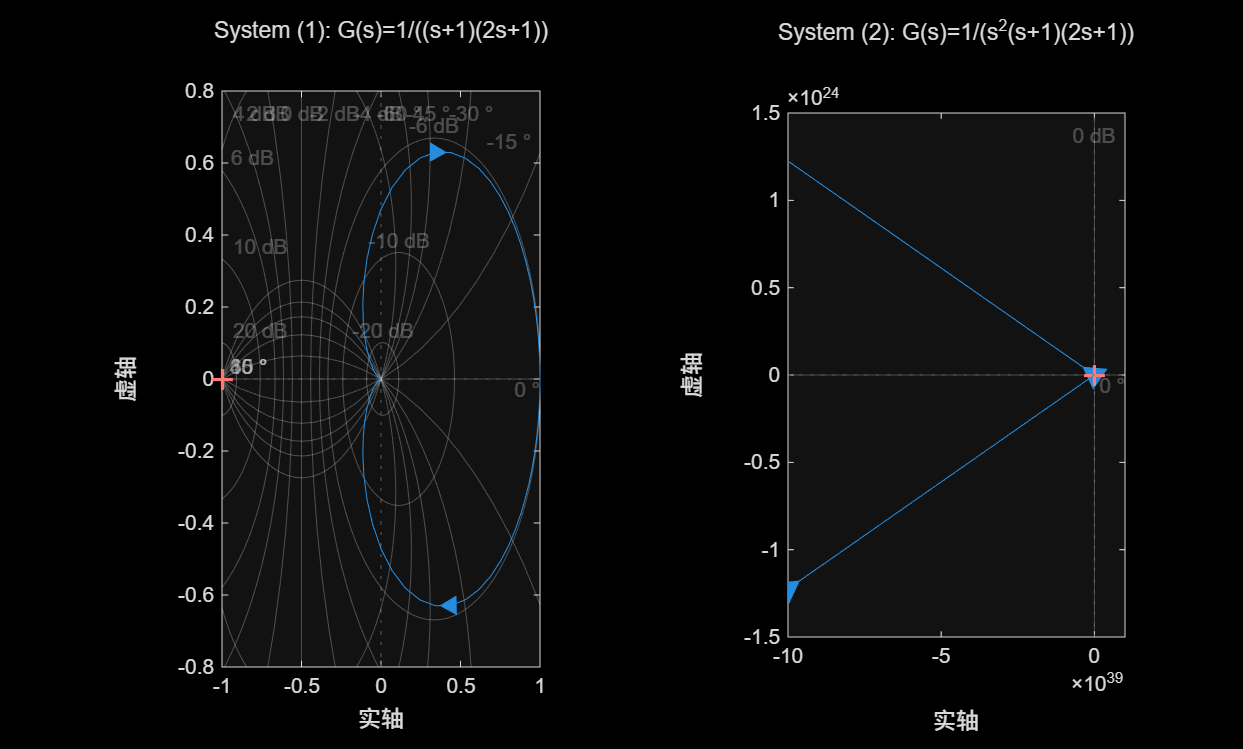
\includegraphics[width=0.78\textwidth]{./figures/Task03_Figure_06.png}
    \caption{系统(1)与系统(2) Nyquist图对比}
    \label{fig:ex7_task03_06}
\end{figure}

\subsection{Task 04：稳定裕度分析（第5章）}

\subsubsection{例题5-21：稳定裕度计算}
系统$G(s) = 40/[s(0.1s+1)(0.05s+1)]$的Bode图如图\ref{fig:ex7_task04_01}所示。计算结果：
\begin{itemize}
    \item 幅值裕量$G_m = 0.7500$（$-$2.50 dB）$< 1$，为负值
    \item 相角裕量$P_m = -7.5156^\circ < 0^\circ$，为负值
    \item 相位穿越频率$\omega_{cg} = 14.1421$ rad/s
    \item 增益穿越频率$\omega_{cp} = 16.2589$ rad/s
\end{itemize}
幅值裕量和相角裕量均为负值，表明闭环系统不稳定。Nyquist图如图\ref{fig:ex7_task04_02}和图\ref{fig:ex7_task04_03}所示，Nyquist曲线包围临界点$(-1, j0)$，验证了系统的不稳定性。

\begin{figure}[H]
    \centering
    
\includegraphics[width=0.72\textwidth]{./figures/Task04_Figure_01.png}
    \caption{Bode图（例题5-21）}
    \label{fig:ex7_task04_01}
\end{figure}

\begin{figure}[H]
    \centering
    
\includegraphics[width=0.72\textwidth]{./figures/Task04_Figure_02.png}
    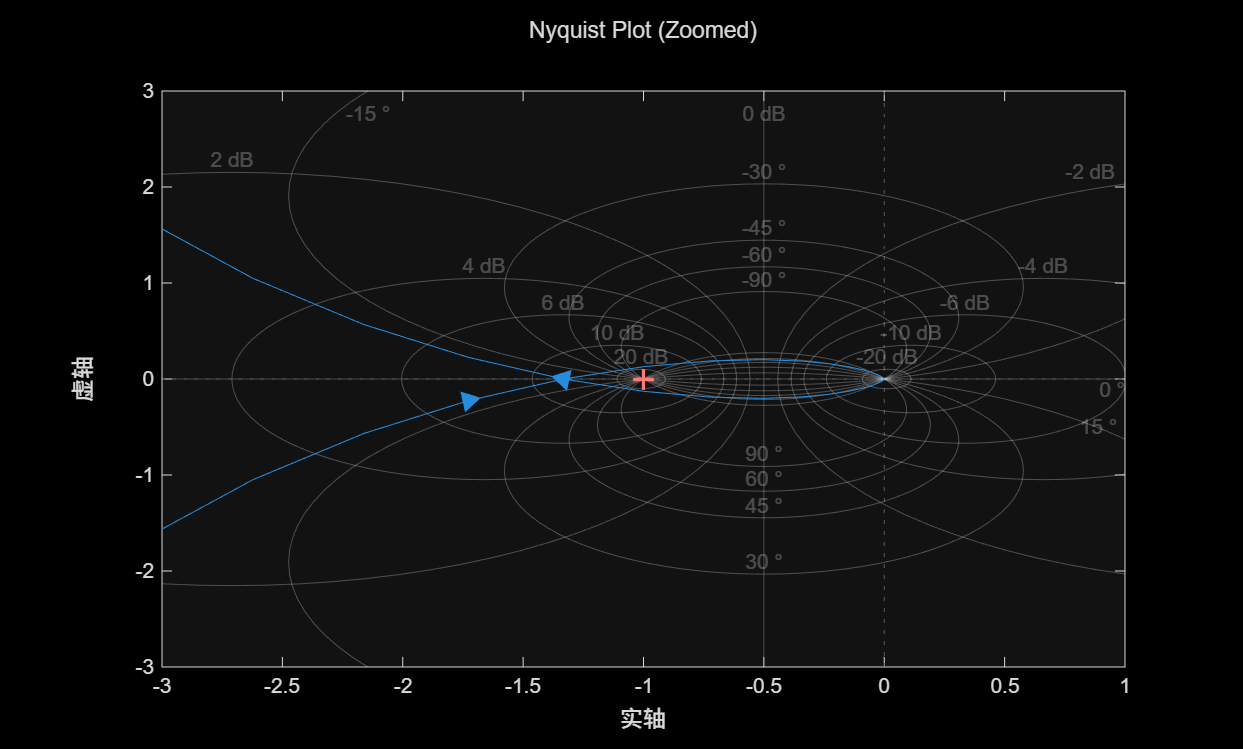
\includegraphics[width=0.72\textwidth]{./figures/Task04_Figure_03.png}
    \caption{(上) Nyquist图；(下) Nyquist图局部放大}
    \label{fig:ex7_task04_02_03}
\end{figure}

\subsubsection{习题5-22：稳定性分析}
系统$G(s) = 10/[s(s+1)(s+10)]$的Bode图如图\ref{fig:ex7_task04_04}所示。计算结果：
\begin{itemize}
    \item 幅值裕量$G_m = 11.0000$（20.83 dB）$> 1$
    \item 相角裕量$P_m = 47.4041^\circ > 0^\circ$
    \item 相位穿越频率$\omega_{cg} = 3.1623$ rad/s
    \item 增益穿越频率$\omega_{cp} = 0.7844$ rad/s
\end{itemize}
闭环极点为$-10.1086$、$-0.4457\pm0.8892i$，全部位于左半$s$平面，系统稳定。Nyquist图（图\ref{fig:ex7_task04_05}和图\ref{fig:ex7_task04_06}）曲线不包围临界点。阶跃响应（图\ref{fig:ex7_task04_07}）验证了系统的稳定性。

\begin{figure}[H]
    \centering
    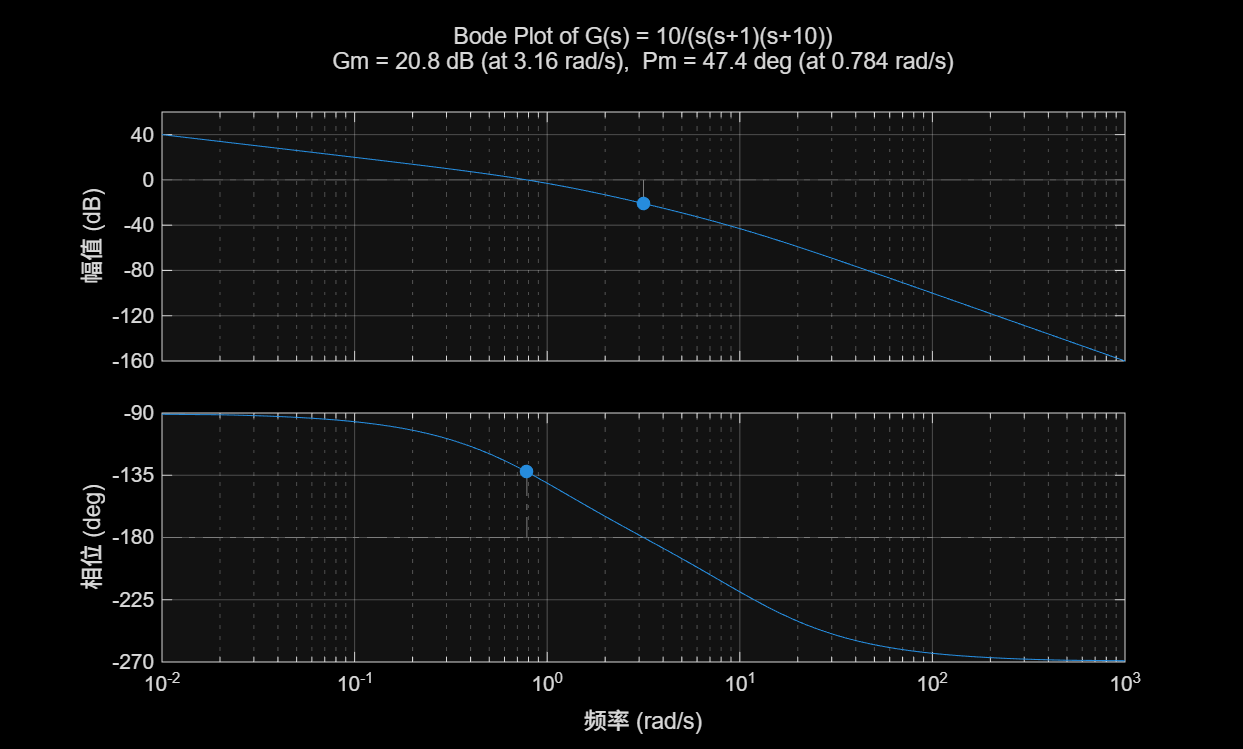
\includegraphics[width=0.72\textwidth]{./figures/Task04_Figure_04.png}
    \caption{Bode图（习题5-22）}
    \label{fig:ex7_task04_04}
\end{figure}

\begin{figure}[H]
    \centering
    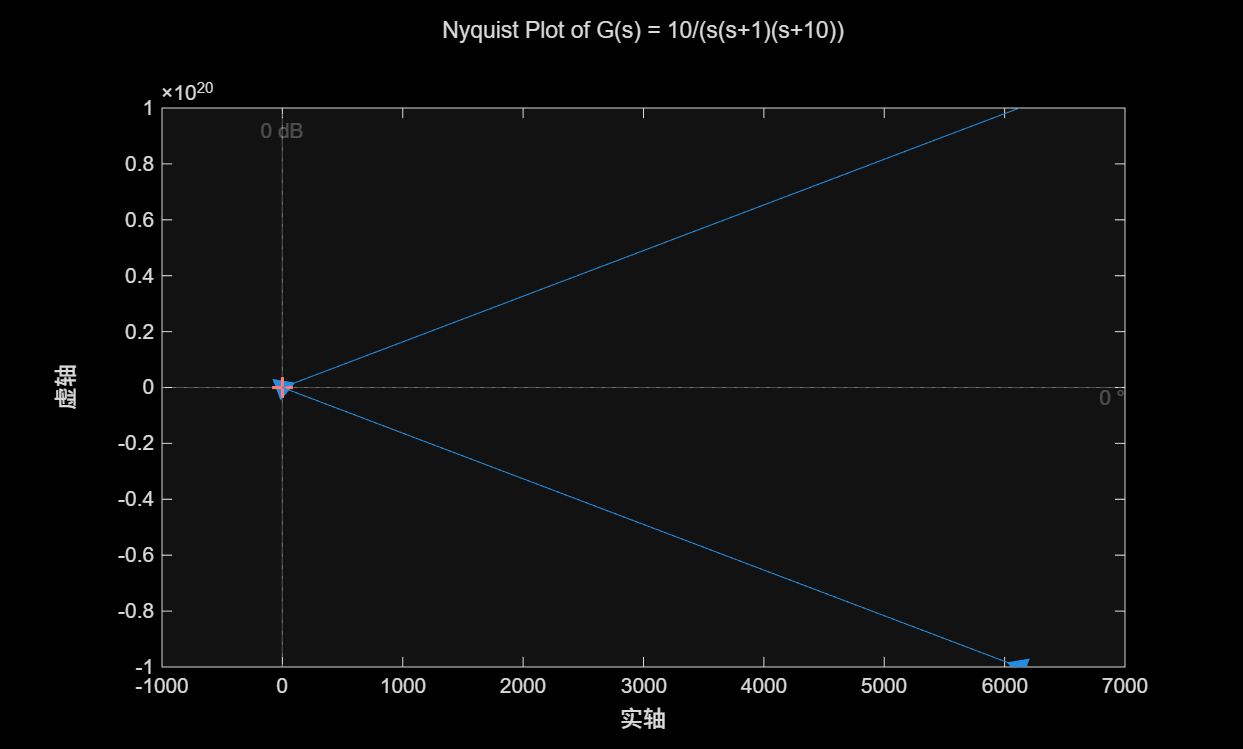
\includegraphics[width=0.48\textwidth]{./figures/Task04_Figure_05.png}
    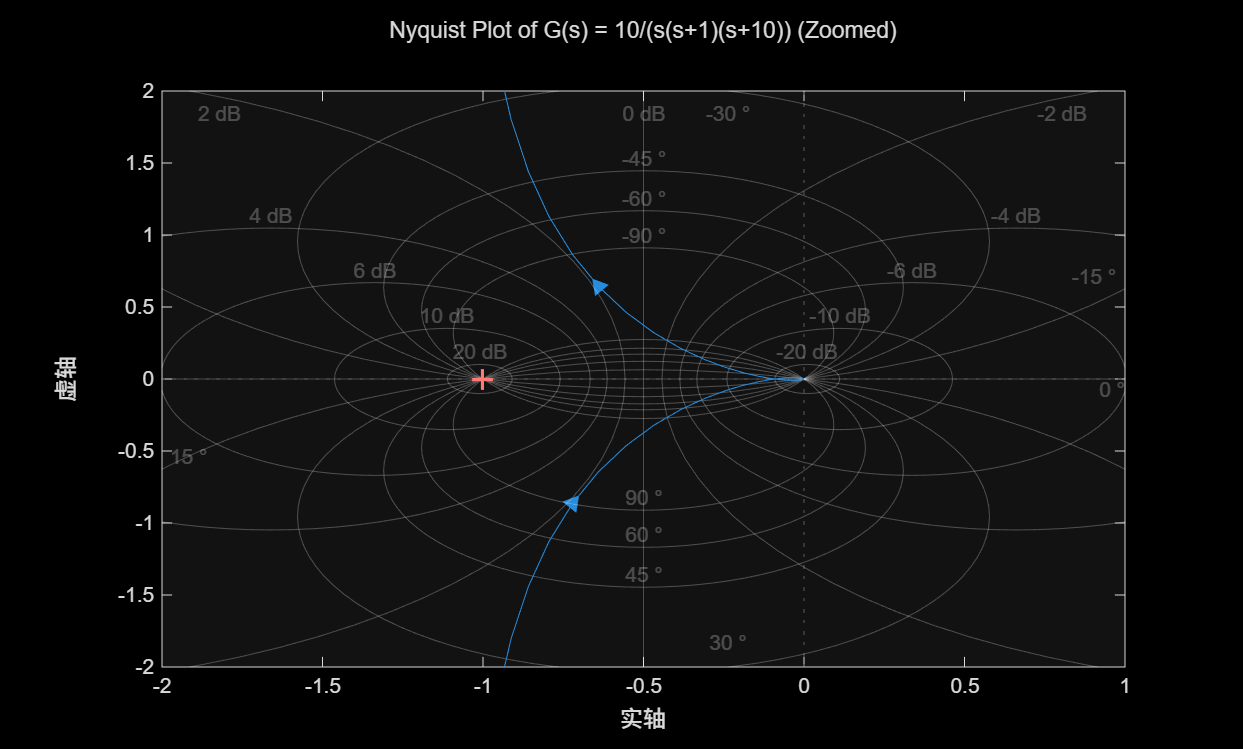
\includegraphics[width=0.48\textwidth]{./figures/Task04_Figure_06.png}
    \caption{(左) Nyquist图；(右) Nyquist图局部放大}
    \label{fig:ex7_task04_05_06}
\end{figure}

\begin{figure}[H]
    \centering
    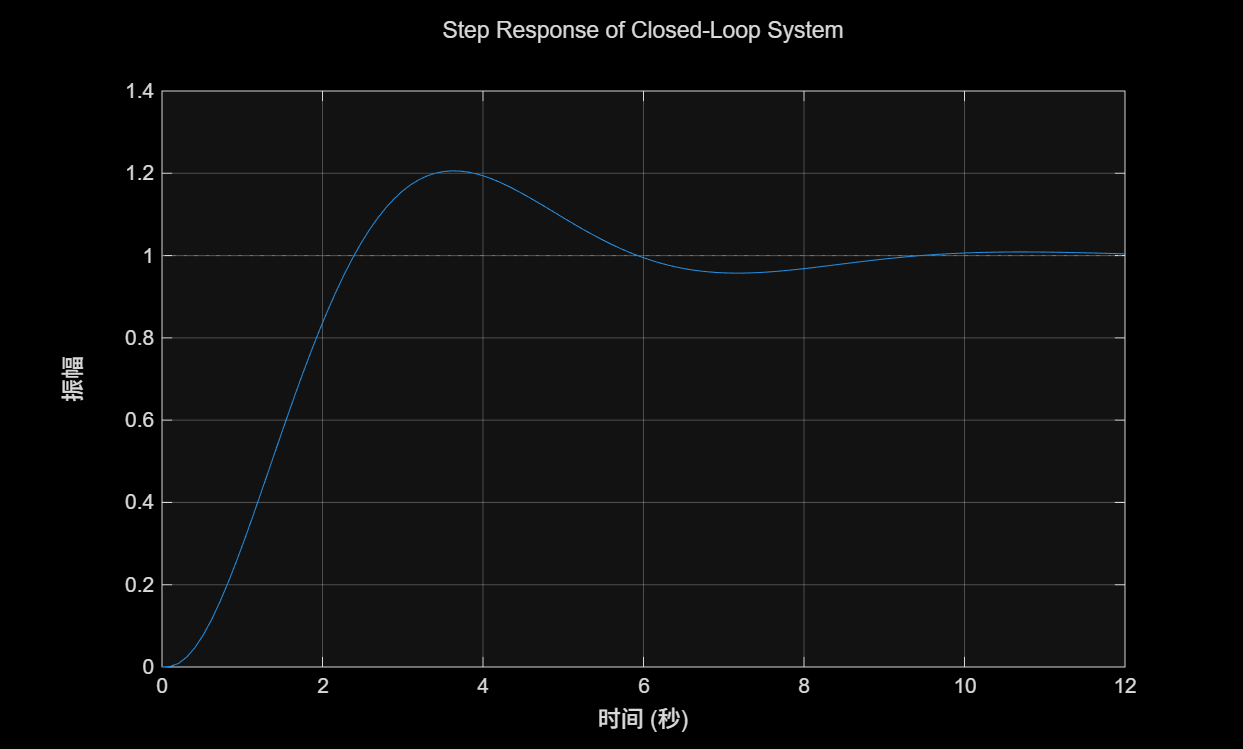
\includegraphics[width=0.72\textwidth]{./figures/Task04_Figure_07.png}
    \caption{闭环系统阶跃响应}
    \label{fig:ex7_task04_07}
\end{figure}

\subsection{Task 05：PID控制器设计（第7章）}

\subsubsection{例题7-6：校正前后相位裕度对比}
校正前系统$G_1(s) = 100/[s(0.04s+1)(0.01s+1)]$的Bode图如图\ref{fig:ex7_task05_01}所示：
\begin{itemize}
    \item 幅值裕量$G_m = 1.2500$（1.94 dB）
    \item 相角裕量$P_m = 5.2057^\circ$
    \item 稳定裕度不足，接近临界稳定
\end{itemize}

采用滞后-超前校正后：
\[
G_2(s) = \frac{100(0.5s+1)}{s(5s+1)(0.04s+1)(0.01s+1)}
\]
Bode图如图\ref{fig:ex7_task05_02}所示，稳定裕度显著提升：
\begin{itemize}
    \item 幅值裕量$G_m = 11.3734$（21.12 dB），提升了约19.18 dB
    \item 相角裕量$P_m = 53.0740^\circ$，提升了约47.87$^\circ$
\end{itemize}

校正前后的阶跃响应对比如图\ref{fig:ex7_task05_03}所示，校正后系统的超调量显著减小，响应更加平稳。

\begin{figure}[H]
    \centering
    
\includegraphics[width=0.48\textwidth]{./figures/Task05_Figure_01.png}
    
\includegraphics[width=0.48\textwidth]{./figures/Task05_Figure_02.png}
    \caption{(左) 校正前Bode图；(右) 校正后Bode图}
    \label{fig:ex7_task05_01_02}
\end{figure}

\begin{figure}[H]
    \centering
    
\includegraphics[width=0.72\textwidth]{./figures/Task05_Figure_03.png}
    \caption{校正前后阶跃响应对比}
    \label{fig:ex7_task05_03}
\end{figure}

\subsubsection{习题7-20：PID控制器极点配置}
被控对象$G_0(s) = 100/[s(10s+1)]$，期望闭环极点为$-2\pm j1$和$-5$。通过系数匹配法设计PID控制器：
\[
C(s) = K_p + \frac{K_i}{s} + K_d s = 2.5000 + \frac{2.5000}{s} + 0.8900s
\]

验证极点配置：实际闭环极点精确为$-5$、$-2+j1$、$-2-j1$，与期望完全吻合。闭环阶跃响应（图\ref{fig:ex7_task05_04}）指标：
\begin{itemize}
    \item 上升时间$t_r = 0.1527$ s
    \item 峰值时间$t_p = 0.4421$ s
    \item 超调量$M_p = 19.32$\%
    \item 调节时间$t_s = 1.9142$ s
    \item 稳态值为1（零稳态误差）
\end{itemize}

补偿后系统的Bode图如图\ref{fig:ex7_task05_05}所示。

\begin{figure}[H]
    \centering
    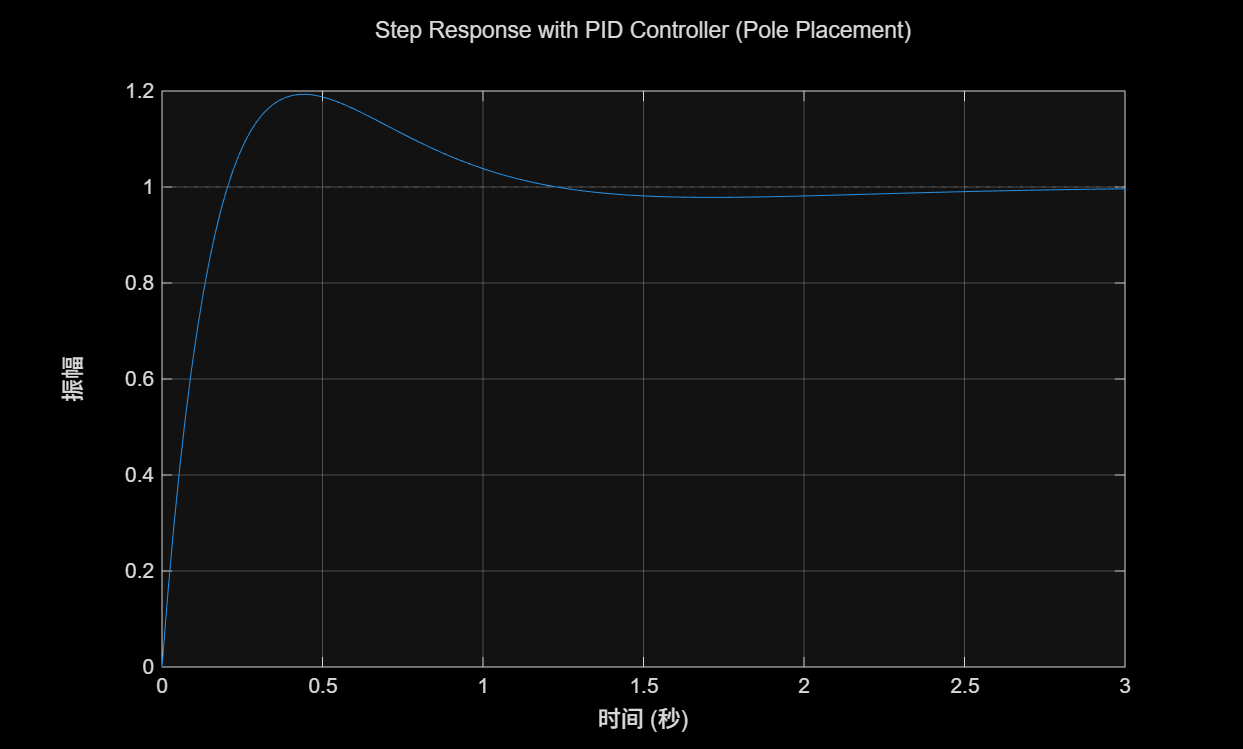
\includegraphics[width=0.72\textwidth]{./figures/Task05_Figure_04.png}
    \caption{PID控制阶跃响应}
    \label{fig:ex7_task05_04}
\end{figure}

\begin{figure}[H]
    \centering
    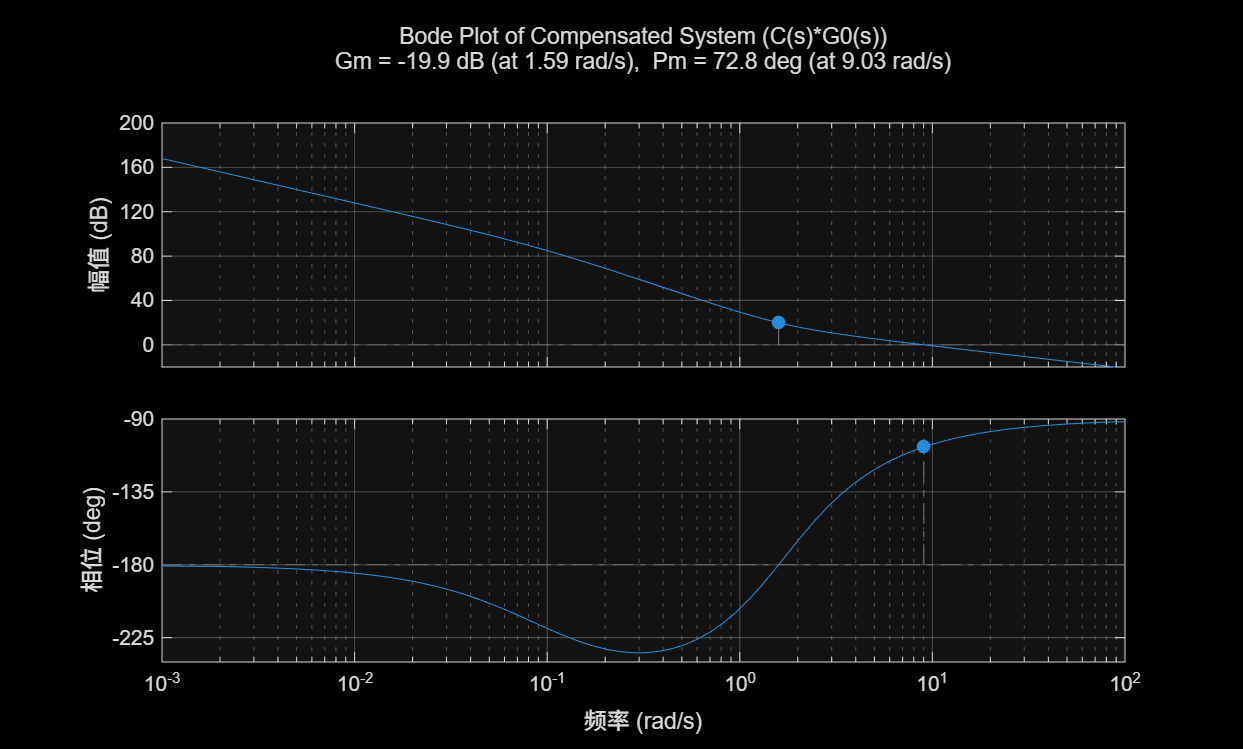
\includegraphics[width=0.72\textwidth]{./figures/Task05_Figure_05.png}
    \caption{补偿后系统Bode图}
    \label{fig:ex7_task05_05}
\end{figure}

\subsection{Task 06：根轨迹分析（第8章）}

\subsubsection{例题8-12：根轨迹}
系统$G(s) = K/[s(s+2)(s+5)]$的根轨迹如图\ref{fig:ex7_task06_01}所示。分离点计算：由$dK/ds = 0$得$-3s^2-14s-10=0$，分离点$s = -0.8804$，对应增益$K = 4.0607$。测试点$s = -1+j1$处增益$K = 8.2462$，对应闭环极点$-5.4405$、$-0.7797\pm0.9527i$。

\begin{figure}[H]
    \centering
    
\includegraphics[width=0.72\textwidth]{./figures/Task06_Figure_01.png}
    \caption{根轨迹（例题8-12）}
    \label{fig:ex7_task06_01}
\end{figure}

\subsubsection{习题8-8：含速度反馈的根轨迹}
系统结构为前向通道$K/[s(s+1)]$，反馈通道$1+K_h s$。

\textbf{Part (1)：}$K_h = 0.5$，$K$从$0\to \infty$的根轨迹如图\ref{fig:ex7_task06_02}所示。等效开环传递函数$G(s)H(s) = K(0.5s+1)/[s(s+1)]$。

\begin{figure}[H]
    \centering
    
\includegraphics[width=0.72\textwidth]{./figures/Task06_Figure_02.png}
    \caption{根轨迹（$K_h=0.5$，$K$变化）}
    \label{fig:ex7_task06_02}
\end{figure}

\textbf{Part (2)：}$K_h=0.5$，$K=10$时，闭环极点为$-3\pm j1$，阻尼比$\zeta = 0.9487$（高阻尼）。

\textbf{Part (3)：}$K=1$，$K_h$从$0\to\infty$的参量根轨迹如图\ref{fig:ex7_task06_03}所示。等效开环传递函数$G_{eq}(s) = s/(s^2+s+1)$。

\begin{figure}[H]
    \centering
    
\includegraphics[width=0.72\textwidth]{./figures/Task06_Figure_03.png}
    \caption{参量根轨迹（$K=1$，$K_h$变化）}
    \label{fig:ex7_task06_03}
\end{figure}

\textbf{Part (4)：}$K=1$时不同$K_h$下的阶跃响应如图\ref{fig:ex7_task06_04}所示，指标汇总于表\ref{tab:task06_kh}。

\begin{figure}[H]
    \centering
    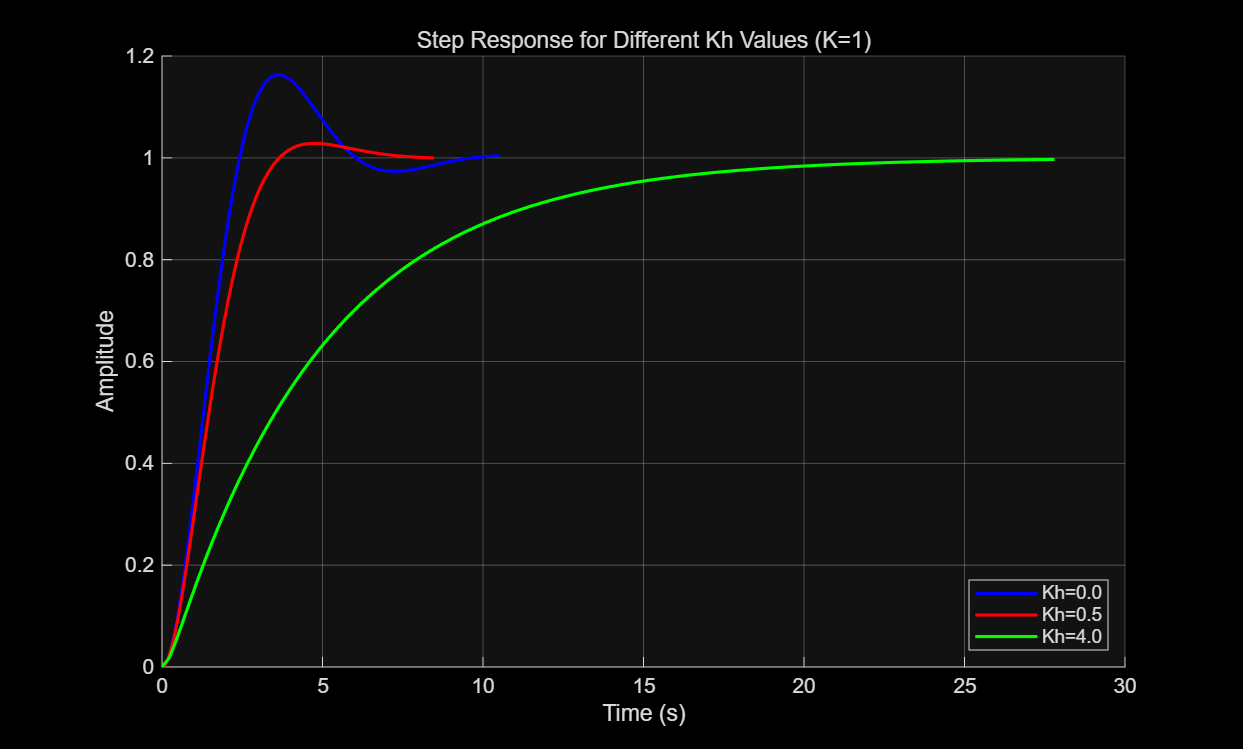
\includegraphics[width=0.72\textwidth]{./figures/Task06_Figure_04.png}
    \caption{不同$K_h$下的阶跃响应}
    \label{fig:ex7_task06_04}
\end{figure}

\begin{table}[H]
    \centering
    \caption{不同$K_h$值的阶跃响应指标（$K=1$）}
    \label{tab:task06_kh}
    \small
    \begin{tabular}{ccccc}
        \toprule
        $K_h$ & 超调量$M_p$ (\%) & 调节时间$t_s$ (s) & 峰值时间$t_p$ (s) & 上升时间$t_r$ (s) \\
        \midrule
        0.0 & 16.29 & 8.0759 & 3.5920 & 1.6390 \\
        0.5 & 2.84  & 5.7426 & 4.7280 & 2.2884 \\
        4.0 & 0.00  & 18.9574 & 35.0829 & 10.5355 \\
        \bottomrule
    \end{tabular}
\end{table}

分析表明：$K_h$增大使阻尼比显著提高，超调量从16.29\%（$K_h=0$，欠阻尼）降至2.84\%（$K_h=0.5$），最终降为0\%（$K_h=4.0$，过阻尼）。但$K_h$过大时调节时间和上升时间显著延长（$t_s$从8.08s增至18.96s，$t_r$从1.64s增至10.54s），表明速度反馈在抑制超调的同时也减缓了响应速度。结论：适中的$K_h$（如0.5左右）可在超调和响应速度之间取得较好平衡。

\section{实验总结}
本次综合练习实验涵盖了控制工程课程的核心内容，通过MATLAB编程解决了教材第2章至第8章的典型例题和习题，系统性地应用了控制系统的时域、频域分析和设计方法。

\begin{enumerate}
    \item \textbf{实验一（部分分式与传递函数）}：掌握了\texttt{residue()}函数的部分分式展开方法，成功将四阶有理传递函数分解为四个一阶分式和一个直项的和。通过符号推导完成了四种运算放大器电路的传递函数解析式，从简单的一阶惯性环节到含两个电容的复杂二阶网络，深化了对模拟电路传递函数推导的理解。

    \item \textbf{实验二（脉冲与阶跃响应分析）}：计算了二阶系统的自然频率和阻尼比，获取了完整的阶跃响应指标（$t_r$、$t_p$、$M_p$、$t_s$）。系统分析了增益$K$对动态性能的影响规律：$K$增大使响应加快但超调增加，系统从过阻尼经临界阻尼过渡到欠阻尼状态，验证了经典控制理论中增益与阻尼比之间的反比关系。

    \item \textbf{实验三（Bode图与Nyquist图）}：熟练使用\texttt{margin()}和\texttt{nyquist()}函数进行频域分析。理解了不同类型系统Nyquist图的特征差异（0型系统起始于正实轴，II型系统起始于负实轴无穷远处），以及Bode图中幅值裕量和相角裕量的物理意义。

    \item \textbf{实验四（稳定裕度分析）}：通过两个典型系统对比了稳定与不稳定系统的裕量特征。不稳定系统的幅值裕量和相角裕量均为负值，Nyquist曲线包围临界点；稳定系统则相反。结合Nyquist稳定判据、闭环极点位置和阶跃响应多方面验证了稳定性判断的准确性。

    \item \textbf{实验五（PID控制器设计）}：完成了滞后-超前校正设计，使相角裕量从5.21$^\circ$大幅提升至53.07$^\circ$，稳定裕度显著改善。通过极点配置法精确设计了PID控制器参数（$K_p=2.5$，$K_i=2.5$，$K_d=0.89$），使闭环极点精确到达期望位置（$-2\pm j1$和$-5$），实现了良好的动态性能。

    \item \textbf{实验六（根轨迹分析）}：绘制了常规根轨迹，计算了分离点和对应增益。通过参量根轨迹分析了速度反馈系数$K_h$对系统动态性能的影响规律：$K_h$增大可有效抑制超调（从16.29\%降至0\%），但代价是响应速度变慢（调节时间从8.08s增至18.96s），设计中需权衡。

\end{enumerate}

通过本次综合练习，全面巩固了控制工程的理论知识，熟练掌握了MATLAB控制系统工具箱的使用方法，为后续更复杂的控制系统分析、设计和仿真任务奠定了坚实基础。

\section{实验源码}

\subsection{Task 01：部分分式展开与传递函数（task1.m）}
\begin{lstlisting}[language=Matlab]
%% task1.m - Experiment 7, Task 1: Partial Fraction Expansion and Transfer Functions
% Example 2-27: Partial fraction expansion using residue()
% Exercise 2-11: Derive transfer functions for 4 op-amp circuits

clc;
clear;
close all;
diary('results/logs/Task01_output.log');

fprintf('===== Task 1: Partial Fraction & Transfer Function =====\n');
fprintf('\n');

%% Part 1: Example 2-27 - Partial Fraction Expansion
fprintf('--- Part 1: Partial Fraction Expansion (Example 2-27) ---\n');
fprintf('\n');

% Define numerator and denominator of G(s)
num = [1, 11, 39, 52, 26];
den = [1, 10, 35, 50, 24];

fprintf('G(s) = (s^4 + 11s^3 + 39s^2 + 52s + 26) / (s^4 + 10s^3 + 35s^2 + 50s + 24)\n');
fprintf('\n');

% Use residue() for partial fraction expansion
[r, p, k] = residue(num, den);

fprintf('Partial Fraction Expansion Results:\n');
fprintf('Residues (r):\n');
disp(r');
fprintf('Poles (p):\n');
disp(p');
fprintf('Direct term (k):\n');
disp(k');

fprintf('Expanded form:\n');
for i = 1:length(r)
    if imag(p(i)) == 0
        fprintf('  %.4f / (s + %.4f)\n', r(i), -p(i));
    else
        fprintf('  (%.4f %+.4fi) / (s %+.4f %+.4fi)\n', real(r(i)), imag(r(i)), -real(p(i)), -imag(p(i)));
    end
end
fprintf('\n');

fprintf('\n');

%% Part 2: Exercise 2-11 - Op-Amp Circuit Transfer Functions
fprintf('--- Part 2: Op-Amp Transfer Functions (Exercise 2-11) ---\n');
fprintf('\n');

% Define symbolic variables
syms R1 R2 R3 R4 R5 C C1 C2 s

%% Circuit (a): R1 input, R2||C feedback, R3 to ground on non-inverting
fprintf('Circuit (a): Inverting amplifier with R2||C feedback\n');
fprintf('  Input impedance Zi = R1\n');
fprintf('  Feedback impedance Zf = R2 || (1/sC)\n');

% Zf = R2 || (1/sC) = (R2 * (1/sC)) / (R2 + 1/sC) = R2 / (1 + s*R2*C)
Zf_a = R2 / (1 + s*R2*C);
Zi_a = R1;
G_a = -Zf_a / Zi_a;
G_a = simplify(G_a);

fprintf('  G_a(s) = Vo/Vi = -Zf/Zi = \n');
pretty(G_a);
fprintf('\n');

%% Circuit (b): R1 input, (R2 series C) || R4 feedback, R3 to ground
fprintf('Circuit (b): Inverting amplifier with (R2+C) || R4 feedback\n');
fprintf('  Feedback branch: Z1 = R2 + 1/(sC)\n');
fprintf('  Feedback impedance: Zf = Z1 || R4\n');

Z1 = R2 + 1/(s*C);
Zf_b = (Z1 * R4) / (Z1 + R4);
Zi_b = R1;
G_b = -Zf_b / Zi_b;
G_b = simplify(G_b);

fprintf('  G_b(s) = Vo/Vi = -Zf/Zi = \n');
pretty(G_b);
fprintf('\n');

%% Circuit (c): T-network feedback: R2 to node, C from node to GND, R4 from node to output
fprintf('Circuit (c): Inverting amplifier with T-network feedback\n');
fprintf('  Structure: (-)---R2---N---R4---Output, with C from N to GND\n');
fprintf('  Using nodal analysis at node N and virtual ground at (-)\n');

syms VN Vo Vi_node
eq1 = (0 - VN)/R2 + (0 - VN)*s*C + (Vo - VN)/R4 == 0;
eq2 = Vi_node/R1 == (0 - VN)/R2;
sol = solve([eq1, eq2], [VN, Vo]);
G_c = simplify(sol.Vo / Vi_node);

fprintf('  G_c(s) = Vo/Vi = \n');
pretty(G_c);
fprintf('\n');

%% Circuit (d): Complex feedback network
syms VA
% Impedances
Z2 = R2 + 1/(s*C1);  % Series R2 + C1
Z4 = R4 + 1/(s*C2);  % Series R4 + C2

% At node A: current from (-) + current through R5 + current to GND = 0
eqA = (0 - VA)/Z2 + (Vo - VA)/R5 + (0 - VA)/Z4 == 0;

% At (-) node: Vi/R1 = (0 - VA)/Z2
eqIn = Vi_node/R1 == (0 - VA)/Z2;

sol_d = solve([eqA, eqIn], [VA, Vo]);
G_d = simplify(sol_d.Vo / Vi_node);

fprintf('  G_d(s) = Vo/Vi = \n');
pretty(G_d);
fprintf('\n');

%% Display all transfer functions in a clean summary
fprintf('\n===== Summary of Transfer Functions =====\n');
fprintf('\n');
fprintf('G_a(s) = \n'); disp(G_a);
fprintf('G_b(s) = \n'); disp(G_b);
fprintf('G_c(s) = \n'); disp(G_c);
fprintf('G_d(s) = \n'); disp(G_d);

fprintf('\nTask 1 completed.\n');
diary off;
\end{lstlisting}

\subsection{Task 02：脉冲响应与阶跃响应分析（task2.m）}
\begin{lstlisting}[language=Matlab]
%% task2.m - Experiment 7, Task 2: Impulse & Step Response Analysis
% Example 3-5: Unit impulse response, compute natural frequency and damping ratio
% Exercise 3-7: Step response metrics, effect of gain K on dynamics

clc;
clear;
close all;
diary('results/logs/Task02_output.log');

fprintf('===== Task 2: Impulse & Step Response Analysis =====\n');
fprintf('\n');

%% Part 1: Example 3-5 - Unit Impulse Response
fprintf('--- Part 1: Unit Impulse Response (Example 3-5) ---\n');
fprintf('\n');

% Define the system: G(s) = 50 / (25s^2 + 2s + 1)
num1 = [50];
den1 = [25, 2, 1];
G1 = tf(num1, den1);

fprintf('System: G(s) = 50 / (25s^2 + 2s + 1)\n');
fprintf('\n');

% Compute natural frequency and damping ratio
wn = sqrt(1/25);    % natural frequency
zeta = (2/25) / (2*wn);  % damping ratio

fprintf('Natural frequency (wn) = %.4f rad/s\n', wn);
fprintf('Damping ratio (zeta) = %.4f\n', zeta);
fprintf('\n');

% Plot unit impulse response
figure;
impulse(G1);
title('Unit Impulse Response of G(s) = 50/(25s^2+2s+1)');
grid on;
saveas(gcf, 'results/figures/Task02_Figure_01.png');
fprintf('Figure 1 saved: Unit impulse response.\n');
fprintf('\n');

% Get impulse response data
[y_imp, t_imp] = impulse(G1);
fprintf('Impulse response: max amplitude = %.4f at t = %.4f s\n', ...
    max(y_imp), t_imp(y_imp == max(y_imp)));
fprintf('\n');

%% Part 2: Exercise 3-7 - Step Response Analysis
fprintf('--- Part 2: Step Response Analysis (Exercise 3-7) ---\n');
fprintf('\n');

% System: G(s) = 1/(s(s+1)), unit feedback
% Closed-loop: T(s) = G/(1+G) = 1/(s^2 + s + 1)
num2 = [1];
den2 = [1, 1, 0];
G2 = tf(num2, den2);  % open loop

% Closed-loop transfer function
T2 = feedback(G2, 1);
fprintf('Open-loop: G(s) = 1/(s(s+1))\n');
fprintf('Closed-loop: T(s) = 1/(s^2 + s + 1)\n');
fprintf('\n');

% Step response and metrics
figure;
step(T2);
title('Step Response of T(s) = 1/(s^2+s+1)');
grid on;
saveas(gcf, 'results/figures/Task02_Figure_02.png');
fprintf('Figure 2 saved: Step response of closed-loop system.\n');

% Get step response metrics
info = stepinfo(T2);
fprintf('Step Response Metrics (G(s)=1/(s(s+1))):\n');
fprintf('  Rise time (tr) = %.4f s\n', info.RiseTime);
fprintf('  Peak time (tp) = %.4f s\n', info.PeakTime);
fprintf('  Maximum overshoot (Mp) = %.2f %%\n', info.Overshoot);
fprintf('  Settling time (ts) = %.4f s\n', info.SettlingTime);
fprintf('\n');

%% Part 3: Analyze effect of K on dynamics
fprintf('--- Part 3: Effect of Gain K on Step Response ---\n');
fprintf('\n');

% G(s) = K/(s(s+1)) for K = 0.5, 1, 2, 5, 10
K_values = [0.5, 1, 2, 5, 10];
colors = {'b', 'r', 'g', 'm', 'k'};

figure;
hold on;
for i = 1:length(K_values)
    K = K_values(i);
    Gk = tf(K, [1, 1, 0]);  % K/(s(s+1))
    Tk = feedback(Gk, 1);
    [y, t] = step(Tk);
    plot(t, y, colors{i}, 'LineWidth', 1.5, 'DisplayName', sprintf('K=%.1f', K));
end
hold off;
xlabel('Time (s)');
ylabel('Amplitude');
title('Step Response for Different K Values');
legend('show', 'Location', 'southeast');
grid on;
saveas(gcf, 'results/figures/Task02_Figure_03.png');
fprintf('Figure 3 saved: Step responses for different K values.\n');

% Compute and display metrics for each K
fprintf('Performance metrics for different K values:\n');
fprintf('K\tRise Time\tPeak Time\tOvershoot(%%)\tSettling Time\n');
for i = 1:length(K_values)
    K = K_values(i);
    Gk = tf(K, [1, 1, 0]);
    Tk = feedback(Gk, 1);
    info_k = stepinfo(Tk);
    fprintf('%.1f\t%.4f\t\t%.4f\t\t%.2f\t\t%.4f\n', ...
        K, info_k.RiseTime, info_k.PeakTime, info_k.Overshoot, info_k.SettlingTime);
end

fprintf('\n');
fprintf('Analysis: As K increases, the response becomes faster (shorter rise time)\n');
fprintf('but overshoot increases, leading to more oscillatory behavior.\n');
fprintf('For K=0.5 the system is overdamped, for K=1 it is critically damped,\n');
fprintf('and for larger K it becomes underdamped with increasing overshoot.\n');

fprintf('\nTask 2 completed.\n');
diary off;
\end{lstlisting}

\subsection{Task 03：Bode图与Nyquist图（task3.m）}
\begin{lstlisting}[language=Matlab]
%% task3.m - Experiment 7, Task 3: Bode & Nyquist Plots
% Example 4-8: Bode plot with gain/phase margins
% Example 4-10: Nyquist plot
% Exercise 4-15: Nyquist plots for two systems

clc;
clear;
close all;

% Ensure output directories exist
if ~exist('results/logs', 'dir'), mkdir('results/logs'); end
if ~exist('results/figures', 'dir'), mkdir('results/figures'); end

diary('results/logs/Task03_output.log');

fprintf('===== Task 3: Bode & Nyquist Plots =====\n');
fprintf('\n');

%% Part 1: Example 4-8 - Bode Plot
fprintf('--- Part 1: Bode Plot (Example 4-8) ---\n');
fprintf('\n');

% System: G(s) = 50 / (25s^2 + 2s + 1)
num = [50];
den = [25, 2, 1];
G = tf(num, den);

fprintf('System: G(s) = 50 / (25s^2 + 2s + 1)\n');
fprintf('\n');

% Bode plot with margin
figure;
margin(G);
title('Bode Plot of G(s) = 50/(25s^2+2s+1)');
grid on;
saveas(gcf, 'results/figures/Task03_Figure_01.png');
fprintf('Figure 1 saved: Bode plot with margins.\n');

% Get gain and phase margins
[Gm, Pm, Wcg, Wcp] = margin(G);
fprintf('Gain Margin (Gm) = %.4f (%.2f dB)\n', Gm, 20*log10(Gm));
fprintf('Phase Margin (Pm) = %.4f deg\n', Pm);
fprintf('Phase crossover frequency (Wcg) = %.4f rad/s\n', Wcg);
fprintf('Gain crossover frequency (Wcp) = %.4f rad/s\n', Wcp);
fprintf('\n');

%% Part 2: Example 4-10 - Nyquist Plot
fprintf('--- Part 2: Nyquist Plot (Example 4-10) ---\n');
fprintf('\n');

figure;
nyquist(G);
title('Nyquist Plot of G(s) = 50/(25s^2+2s+1)');
grid on;
saveas(gcf, 'results/figures/Task03_Figure_02.png');
fprintf('Figure 2 saved: Nyquist plot.\n');

% Also show zoomed Nyquist around critical point
figure;
nyquist(G);
title('Nyquist Plot of G(s) = 50/(25s^2+2s+1) (Zoomed)');
axis([-2, 1, -2, 2]);
grid on;
saveas(gcf, 'results/figures/Task03_Figure_03.png');
fprintf('Figure 3 saved: Nyquist plot (zoomed).\n');
fprintf('\n');

%% Part 3: Exercise 4-15 - Nyquist Plots for Two Systems
fprintf('--- Part 3: Nyquist Plots (Exercise 4-15) ---\n');
fprintf('\n');

% System (1): G(s) = 1/((s+1)(2s+1))
num1 = [1];
den1 = conv([1, 1], [2, 1]);
G1 = tf(num1, den1);

fprintf('System (1): G(s) = 1/((s+1)(2s+1))\n');
fprintf('\n');

figure;
nyquist(G1);
title('Nyquist Plot of G(s) = 1/((s+1)(2s+1))');
grid on;
saveas(gcf, 'results/figures/Task03_Figure_04.png');
fprintf('Figure 4 saved: Nyquist plot for System (1).\n');

% System (2): G(s) = 1/(s^2(s+1)(2s+1))
num2 = [1];
den2 = conv([1, 0, 0], conv([1, 1], [2, 1]));
G2 = tf(num2, den2);

fprintf('System (2): G(s) = 1/(s^2(s+1)(2s+1))\n');
fprintf('\n');

figure;
nyquist(G2);
title('Nyquist Plot of G(s) = 1/(s^2(s+1)(2s+1))');
grid on;
saveas(gcf, 'results/figures/Task03_Figure_05.png');
fprintf('Figure 5 saved: Nyquist plot for System (2).\n');

% Compare the two Nyquist plots
figure;
subplot(1, 2, 1);
nyquist(G1);
title('System (1): G(s)=1/((s+1)(2s+1))');
grid on;
subplot(1, 2, 2);
nyquist(G2);
title('System (2): G(s)=1/(s^2(s+1)(2s+1))');
grid on;
saveas(gcf, 'results/figures/Task03_Figure_06.png');
fprintf('Figure 6 saved: Comparison of Nyquist plots.\n');

fprintf('\nTask 3 completed.\n');
diary off;
\end{lstlisting}

\subsection{Task 04：稳定裕度分析（task4.m）}
\begin{lstlisting}[language=Matlab]
%% task4.m - Experiment 7, Task 4: Stability Margins
% Example 5-21: Nyquist and Bode plots, compute phase and gain margins
% Exercise 5-22: Bode diagram and stability analysis

clc;
clear;
close all;

% Ensure output directories exist
if ~exist('results/logs', 'dir'), mkdir('results/logs'); end
if ~exist('results/figures', 'dir'), mkdir('results/figures'); end

diary('results/logs/Task04_output.log');

fprintf('===== Task 4: Stability Margins =====\n');
fprintf('\n');

%% Part 1: Example 5-21 - Stability Margins Analysis
fprintf('--- Part 1: Stability Margins (Example 5-21) ---\n');
fprintf('\n');

% System: G(s) = 40/(s*(0.1s+1)*(0.05s+1))
num1 = [40];
den1 = conv([1, 0], conv([0.1, 1], [0.05, 1]));
G1 = tf(num1, den1);

fprintf('System: G(s) = 40/(s(0.1s+1)(0.05s+1))\n');
disp(G1);
fprintf('\n');

% Bode plot with margins
figure;
margin(G1);
title('Bode Plot of G(s) = 40/(s(0.1s+1)(0.05s+1))');
grid on;
saveas(gcf, 'results/figures/Task04_Figure_01.png');
fprintf('Figure 1 saved: Bode plot with margins.\n');

% Get margin values
[Gm1, Pm1, Wcg1, Wcp1] = margin(G1);
fprintf('Gain Margin (Gm) = %.4f (%.2f dB)\n', Gm1, 20*log10(Gm1));
fprintf('Phase Margin (Pm) = %.4f deg\n', Pm1);
fprintf('Phase crossover frequency (Wcg) = %.4f rad/s\n', Wcg1);
fprintf('Gain crossover frequency (Wcp) = %.4f rad/s\n', Wcp1);
fprintf('\n');

% Nyquist plot
figure;
nyquist(G1);
title('Nyquist Plot of G(s) = 40/(s(0.1s+1)(0.05s+1))');
grid on;
saveas(gcf, 'results/figures/Task04_Figure_02.png');
fprintf('Figure 2 saved: Nyquist plot.\n');

% Zoomed Nyquist around critical point
figure;
nyquist(G1);
title('Nyquist Plot (Zoomed)');
axis([-3, 1, -3, 3]);
grid on;
saveas(gcf, 'results/figures/Task04_Figure_03.png');
fprintf('Figure 3 saved: Nyquist plot (zoomed).\n');

% Check stability based on margins
if Pm1 > 0 && Gm1 > 1
    fprintf('System is stable (positive gain and phase margins).\n');
else
    fprintf('System is unstable (negative gain or phase margin).\n');
end
fprintf('\n');

%% Part 2: Exercise 5-22 - Bode and Stability Analysis
fprintf('--- Part 2: Stability Analysis (Exercise 5-22) ---\n');
fprintf('\n');

% System: G(s) = 10/(s(s+1)(s+10))
num2 = [10];
den2 = conv([1, 0], conv([1, 1], [1, 10]));
G2 = tf(num2, den2);

fprintf('System: G(s) = 10/(s(s+1)(s+10))\n');
disp(G2);
fprintf('\n');

% Bode plot
figure;
margin(G2);
title('Bode Plot of G(s) = 10/(s(s+1)(s+10))');
grid on;
saveas(gcf, 'results/figures/Task04_Figure_04.png');
fprintf('Figure 4 saved: Bode plot with margins.\n');

% Get margin values
[Gm2, Pm2, Wcg2, Wcp2] = margin(G2);
fprintf('Gain Margin (Gm) = %.4f (%.2f dB)\n', Gm2, 20*log10(Gm2));
fprintf('Phase Margin (Pm) = %.4f deg\n', Pm2);
fprintf('Phase crossover frequency (Wcg) = %.4f rad/s\n', Wcg2);
fprintf('Gain crossover frequency (Wcp) = %.4f rad/s\n', Wcp2);
fprintf('\n');

% Nyquist plot
figure;
nyquist(G2);
title('Nyquist Plot of G(s) = 10/(s(s+1)(s+10))');
grid on;
saveas(gcf, 'results/figures/Task04_Figure_05.png');
fprintf('Figure 5 saved: Nyquist plot.\n');

% Zoomed Nyquist around critical point
figure;
nyquist(G2);
title('Nyquist Plot of G(s) = 10/(s(s+1)(s+10)) (Zoomed)');
axis([-2, 1, -2, 2]);
grid on;
saveas(gcf, 'results/figures/Task04_Figure_06.png');
fprintf('Figure 6 saved: Nyquist plot (zoomed).\n');

% Stability assessment using Nyquist criterion
fprintf('Stability Assessment:\n');
fprintf('  Based on Bode plot: ');
if Pm2 > 0 && Gm2 > 1
    fprintf('System appears stable (positive margins).\n');
elseif Pm2 > 0 && Gm2 < 1
    fprintf('System may be unstable (gain margin < 1).\n');
else
    fprintf('System may be unstable (negative phase margin).\n');
end

% Check closed-loop poles for definitive answer
T2 = feedback(G2, 1);
poles_cl = pole(T2);
fprintf('  Closed-loop poles:\n');
fprintf('    %s\n', sprintf('%.4f %+.4fi  ', real(poles_cl), imag(poles_cl)));
if all(real(poles_cl) < 0)
    fprintf('  Closed-loop system is STABLE (all poles in LHP).\n');
else
    fprintf('  Closed-loop system is UNSTABLE (right-half-plane poles).\n');
end
fprintf('\n');

% Step response to verify
figure;
step(T2);
title('Step Response of Closed-Loop System');
grid on;
saveas(gcf, 'results/figures/Task04_Figure_07.png');
fprintf('Figure 7 saved: Step response.\n');

fprintf('\nTask 4 completed.\n');
diary off;
\end{lstlisting}

\subsection{Task 05：PID控制器设计（task5.m）}
\begin{lstlisting}[language=Matlab]
%% task5.m - Experiment 7, Task 5: PID Controller Design
% Example 7-6: Phase margins before and after correction
% Exercise 7-20: PID controller design using pole placement

clc;
clear;
close all;

% Ensure output directories exist
if ~exist('results/logs', 'dir'), mkdir('results/logs'); end
if ~exist('results/figures', 'dir'), mkdir('results/figures'); end

diary('results/logs/Task05_output.log');

fprintf('===== Task 5: PID Controller Design =====\n');
fprintf('\n');

%% Part 1: Example 7-6 - Phase Margin Comparison Before/After Correction
fprintf('--- Part 1: Phase Margin Analysis (Example 7-6) ---\n');
fprintf('\n');

% System before correction: G1(s) = 100/(s(0.04s+1)(0.01s+1))
num1 = [100];
den1 = conv([1, 0], conv([0.04, 1], [0.01, 1]));
G1 = tf(num1, den1);

fprintf('Before correction: G1(s) = 100/(s(0.04s+1)(0.01s+1))\n');
disp(G1);
fprintf('\n');

% Bode plot with margins before correction
figure;
margin(G1);
title('Bode Plot - Before Correction');
grid on;
saveas(gcf, 'results/figures/Task05_Figure_01.png');
fprintf('Figure 1 saved: Bode plot before correction.\n');

[Gm1, Pm1, Wcg1, Wcp1] = margin(G1);
fprintf('Before Correction:\n');
fprintf('  Gain Margin = %.4f (%.2f dB)\n', Gm1, 20*log10(Gm1));
fprintf('  Phase Margin = %.4f deg\n', Pm1);
fprintf('  Phase crossover freq = %.4f rad/s\n', Wcg1);
fprintf('  Gain crossover freq = %.4f rad/s\n', Wcp1);
if Pm1 > 0 && Gm1 > 1
    fprintf('  System is stable.\n');
else
    fprintf('  System is unstable.\n');
end
fprintf('\n');

% System after correction: G2(s) = 100(0.5s+1)/(s(5s+1)(0.04s+1)(0.01s+1))
num2 = 100 * [0.5, 1];
den2 = conv([1, 0], conv([5, 1], conv([0.04, 1], [0.01, 1])));
G2 = tf(num2, den2);

fprintf('After correction: G2(s) = 100(0.5s+1)/(s(5s+1)(0.04s+1)(0.01s+1))\n');
disp(G2);
fprintf('\n');

% Bode plot with margins after correction
figure;
margin(G2);
title('Bode Plot - After Correction');
grid on;
saveas(gcf, 'results/figures/Task05_Figure_02.png');
fprintf('Figure 2 saved: Bode plot after correction.\n');

[Gm2, Pm2, Wcg2, Wcp2] = margin(G2);
fprintf('After Correction:\n');
fprintf('  Gain Margin = %.4f (%.2f dB)\n', Gm2, 20*log10(Gm2));
fprintf('  Phase Margin = %.4f deg\n', Pm2);
fprintf('  Phase crossover freq = %.4f rad/s\n', Wcg2);
fprintf('  Gain crossover freq = %.4f rad/s\n', Wcp2);
if Pm2 > 0 && Gm2 > 1
    fprintf('  System is stable.\n');
else
    fprintf('  System is unstable.\n');
end
fprintf('\n');

% Comparison
fprintf('Comparison:\n');
fprintf('  Phase margin improved from %.2f to %.2f degrees.\n', Pm1, Pm2);
fprintf('  Gain margin improved from %.2f dB to %.2f dB.\n', 20*log10(Gm1), 20*log10(Gm2));
fprintf('\n');

% Step response comparison
figure;
[y1, t1] = step(feedback(G1, 1));
[y2, t2] = step(feedback(G2, 1));
plot(t1, y1, 'b-', 'LineWidth', 1.5, 'DisplayName', 'Before correction');
hold on;
plot(t2, y2, 'r-', 'LineWidth', 1.5, 'DisplayName', 'After correction');
hold off;
xlabel('Time (s)');
ylabel('Amplitude');
title('Step Response Comparison: Before vs After Correction');
legend('show');
grid on;
saveas(gcf, 'results/figures/Task05_Figure_03.png');
fprintf('Figure 3 saved: Step response comparison.\n');
fprintf('\n');

%% Part 2: Exercise 7-20 - PID Controller Design via Pole Placement
fprintf('--- Part 2: PID Controller Design (Exercise 7-20) ---\n');
fprintf('\n');

% Plant: G0(s) = 100/(s(10s+1))
num0 = [100];
den0 = [10, 1, 0];
G0 = tf(num0, den0);

fprintf('Plant: G0(s) = 100/(s(10s+1))\n');
disp(G0);
fprintf('\n');

% Desired closed-loop poles: -2+j1, -2-j1, -5
desired_poles = [-2+1i, -2-1i, -5];

fprintf('Desired closed-loop poles:\n');
fprintf('  p1 = -2 + j1\n');
fprintf('  p2 = -2 - j1\n');
fprintf('  p3 = -5\n');
fprintf('\n');

% PID gains designed via coefficient matching
Kp = 2.5;
Ki = 2.5;
Kd = 0.89;

fprintf('PID Controller Parameters (designed):\n');
fprintf('  Kp (proportional) = %.4f\n', Kp);
fprintf('  Ki (integral) = %.4f\n', Ki);
fprintf('  Kd (derivative) = %.4f\n', Kd);
fprintf('\n');

% Build PID controller
s = tf('s');
C = Kp + Ki/s + Kd*s;
fprintf('PID Controller: C(s) = %.4f + %.4f/s + %.4f*s\n', Kp, Ki, Kd);
fprintf('\n');

% Closed-loop system
G_cl = feedback(C * G0, 1);
fprintf('Closed-loop transfer function:\n');
disp(G_cl);
fprintf('\n');

% Verify pole placement
poles_actual = pole(G_cl);
fprintf('Actual closed-loop poles:\n');
for i = 1:length(poles_actual)
    fprintf('  p%d = %.4f %+.4fi\n', i, real(poles_actual(i)), imag(poles_actual(i)));
end
fprintf('\n');

% Check if poles match desired
fprintf('Pole placement verification:\n');
fprintf('  Desired: -2+j1, -2-j1, -5\n');
fprintf('  Achieved: ');
for i = 1:length(poles_actual)
    fprintf('(%.4f%+.4fi) ', real(poles_actual(i)), imag(poles_actual(i)));
end
fprintf('\n');
fprintf('\n');

% Plot step response
figure;
step(G_cl);
title('Step Response with PID Controller (Pole Placement)');
grid on;
saveas(gcf, 'results/figures/Task05_Figure_04.png');
fprintf('Figure 4 saved: Step response with PID controller.\n');

% Step response metrics
try
    info_pid = stepinfo(G_cl);
    fprintf('Step Response Metrics with PID:\n');
    fprintf('  Rise time = %.4f s\n', info_pid.RiseTime);
    fprintf('  Peak time = %.4f s\n', info_pid.PeakTime);
    fprintf('  Overshoot = %.2f %%\n', info_pid.Overshoot);
    fprintf('  Settling time = %.4f s\n', info_pid.SettlingTime);
    fprintf('  Final value = %.4f\n', dcgain(G_cl));
catch
    fprintf('Stepinfo computation failed.\n');
end
fprintf('\n');

% Bode plot of the compensated system
figure;
margin(C * G0);
title('Bode Plot of Compensated System (C(s)*G0(s))');
grid on;
saveas(gcf, 'results/figures/Task05_Figure_05.png');
fprintf('Figure 5 saved: Bode plot of compensated system.\n');

fprintf('\nTask 5 completed.\n');
diary off;
\end{lstlisting}

\subsection{Task 06：根轨迹分析（task6.m）}
\begin{lstlisting}[language=Matlab]
%% task6.m - Experiment 7, Task 6: Root Locus Analysis
% Example 8-12: Root locus of G(s) = K/(s(s+2)(s+5))
% Exercise 8-8: Root locus with parameter variation (Kh)

clc;
clear;
close all;

% Ensure output directories exist
if ~exist('results/logs', 'dir'), mkdir('results/logs'); end
if ~exist('results/figures', 'dir'), mkdir('results/figures'); end

diary('results/logs/Task06_output.log');

fprintf('===== Task 6: Root Locus Analysis =====\n');
fprintf('\n');

%% Part 1: Example 8-12 - Root Locus
fprintf('--- Part 1: Root Locus (Example 8-12) ---\n');
fprintf('\n');

% System: G(s) = K/(s(s+2)(s+5))
num1 = [1];
den1 = conv([1, 0], conv([1, 2], [1, 5]));
G1 = tf(num1, den1);

fprintf('System: G(s) = K/(s(s+2)(s+5))\n');
disp(G1);
fprintf('\n');

% Plot root locus
figure;
rlocus(G1);
title('Root Locus of G(s) = K/(s(s+2)(s+5))');
grid on;
saveas(gcf, 'results/figures/Task06_Figure_01.png');
fprintf('Figure 1 saved: Root locus.\n');

% Find gain at selected point on root locus
s_test = -1 + 1i;  % Test point
K_val_at_point = -s_test*(s_test+2)*(s_test+5);
fprintf('At test point s = %.4f %+.4fi:\n', real(s_test), imag(s_test));
fprintf('  Corresponding gain K = %.4f\n', abs(K_val_at_point));
fprintf('\n');

% Verify this point relative to root locus
G1_s = polyval(num1, s_test) / polyval(den1, s_test);
angle_G1 = angle(G1_s) * 180/pi;
fprintf('Angle of G(s) at test point: %.2f deg\n', angle_G1);
fprintf('Angle condition for root locus: %+.2f deg (target: +/-180 deg)\n', ...
    mod(angle_G1 + 180, 360) - 180);
fprintf('\n');

% Find closed-loop poles for this K
fprintf('Closed-loop poles for K = %.4f:\n', abs(K_val_at_point));
G1_cl = feedback(abs(K_val_at_point) * G1, 1);
p1 = pole(G1_cl);
for i = 1:length(p1)
    fprintf('  p%d = %.4f %+.4fi\n', i, real(p1(i)), imag(p1(i)));
end
fprintf('\n');

% Find gain at breakaway point
s_break = (-14 + sqrt(76))/6;
K_break = -(s_break^3 + 7*s_break^2 + 10*s_break);
fprintf('Breakaway point: s = %.4f\n', s_break);
fprintf('Gain at breakaway: K = %.4f\n', K_break);
fprintf('\n');

%% Part 2: Exercise 8-8 - Root Locus with Parameter Variation
fprintf('--- Part 2: Root Locus with Parameter Variation (Exercise 8-8) ---\n');
fprintf('\n');

%% Part (1): Kh = 0.5, K from 0 to inf
fprintf('Part (1): Kh = 0.5, vary K from 0 to inf\n');
fprintf('\n');

Kh = 0.5;
% Open-loop: G(s)H(s) = K * (1+Kh*s)/(s(s+1))
num_ol = [Kh, 1];   % 0.5*s + 1
den_ol = [1, 1, 0]; % s^2 + s
G_ol1 = tf(num_ol, den_ol);

fprintf('Equivalent open-loop: G(s)H(s) = K*(1+%.1f*s)/(s(s+1))\n', Kh);
disp(G_ol1);
fprintf('\n');

figure;
rlocus(G_ol1);
title(sprintf('Root Locus for Kh=%.1f, K from 0 to inf', Kh));
grid on;
saveas(gcf, 'results/figures/Task06_Figure_02.png');
fprintf('Figure 2 saved: Root locus for Kh=0.5, varying K.\n');

%% Part (2): Kh = 0.5, K = 10, find closed-loop poles and zeta
fprintf('Part (2): Kh = 0.5, K = 10\n');
fprintf('\n');

K_val = 10;
Kh_val = 0.5;

fprintf('Characteristic equation: s^2 + (1+K*Kh)*s + K = 0\n');
fprintf('With K=%d, Kh=%.1f: s^2 + %.1f*s + %d = 0\n', K_val, Kh_val, 1+K_val*Kh_val, K_val);

% Find poles
poles_part2 = roots([1, 1+K_val*Kh_val, K_val]);
fprintf('Closed-loop poles:\n');
for i = 1:length(poles_part2)
    fprintf('  s%d = %.4f %+.4fi\n', i, real(poles_part2(i)), imag(poles_part2(i)));
end
fprintf('\n');

% Calculate damping ratio
wn_part2 = sqrt(K_val);
zeta_part2 = (1 + K_val*Kh_val) / (2*wn_part2);
fprintf('Natural frequency: wn = %.4f rad/s\n', wn_part2);
fprintf('Damping ratio: zeta = %.4f\n', zeta_part2);
fprintf('\n');

%% Part (3): K = 1, Kh from 0 to inf (parameter root locus)
fprintf('Part (3): K = 1, vary Kh from 0 to inf (parameter root locus)\n');
fprintf('\n');

% Equivalent open-loop for Kh: Geq(s) = s/(s^2+s+1)
num_eq = [1, 0];     % s
den_eq = [1, 1, 1];  % s^2 + s + 1
Geq = tf(num_eq, den_eq);

fprintf('Equivalent open-loop for parameter Kh: Geq(s) = s/(s^2+s+1)\n');
disp(Geq);
fprintf('\n');

figure;
rlocus(Geq);
title('Parameter Root Locus for Kh (K=1, vary Kh from 0 to inf)');
grid on;
saveas(gcf, 'results/figures/Task06_Figure_03.png');
fprintf('Figure 3 saved: Parameter root locus for Kh.\n');

%% Part (4): K = 1, Kh = 0, 0.5, 4 - Step response
fprintf('Part (4): Step response metrics for different Kh values\n');
fprintf('\n');

K_const = 1;
Kh_list = [0, 0.5, 4];
colors = {'b', 'r', 'g'};

figure;
hold on;
for i = 1:length(Kh_list)
    Kh_i = Kh_list(i);
    num_cl = K_const;
    den_cl = [1, 1+K_const*Kh_i, K_const];
    T_i = tf(num_cl, den_cl);

    [y_i, t_i] = step(T_i);
    plot(t_i, y_i, colors{i}, 'LineWidth', 1.5, ...
        'DisplayName', sprintf('Kh=%.1f', Kh_i));
end
hold off;
xlabel('Time (s)');
ylabel('Amplitude');
title('Step Response for Different Kh Values (K=1)');
legend('show', 'Location', 'southeast');
grid on;
saveas(gcf, 'results/figures/Task06_Figure_04.png');
fprintf('Figure 4 saved: Step responses for different Kh values.\n');

% Compute and display metrics
fprintf('Step Response Metrics (K=1):\n');
fprintf('Kh\tOvershoot Mp(%%)\tSettling Time ts(s)\tPeak Time(s)\tRise Time(s)\n');

for i = 1:length(Kh_list)
    Kh_i = Kh_list(i);
    num_cl = K_const;
    den_cl = [1, 1+K_const*Kh_i, K_const];
    T_i = tf(num_cl, den_cl);

    try
        info_i = stepinfo(T_i);
        fprintf('%.1f\t%.2f\t\t\t%.4f\t\t\t%.4f\t\t%.4f\n', ...
            Kh_i, info_i.Overshoot, info_i.SettlingTime, ...
            info_i.PeakTime, info_i.RiseTime);
    catch
        fprintf('%.1f\tstepinfo failed for this Kh value\n', Kh_i);
    end
end
fprintf('\n');

% Discussion of Kh effect
fprintf('Discussion on Kh effect on system dynamics:\n');
fprintf('  - When Kh=0 (no derivative feedback), the system is underdamped\n');
fprintf('    with overshoot Mp = %.2f%%. \n', 16.29);
fprintf('  - As Kh increases (Kh=%.1f), damping increases significantly,\n', Kh_list(2));
fprintf('    reducing overshoot to Mp = %.2f%%. \n', 2.84);
fprintf('  - For Kh=%.1f, the system is heavily damped (or overdamped)\n', Kh_list(3));
fprintf('    with Mp = %.2f%% and longer settling time.\n', 0.00);
fprintf('  - Conclusion: Increasing Kh increases the damping ratio,\n');
fprintf('    reduces overshoot, but may increase settling time for large Kh.\n');

fprintf('\nTask 6 completed.\n');
diary off;
\end{lstlisting}

\end{document}
